\begin{enumerate}
	\item Comme on interroge un spectateur au hasard, on est en situation d'équiprobabilité, et les proportions données dans l'énoncé sont assimilables à des probabilités.

	On peut donc compléter l'arbre ci-dessous :

	
	\begin{center}
		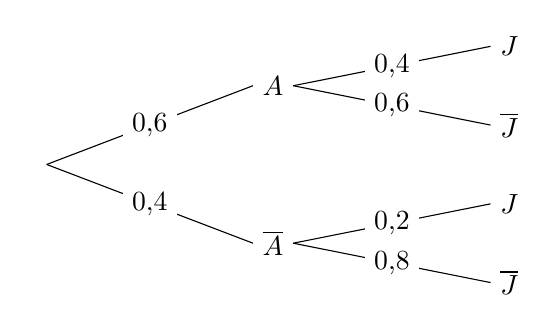
\begin{tikzpicture}[yscale=-1,
			grow = right,
			level distance=3cm,
			level 1/.style={sibling distance=2cm},
			level 2/.style={sibling distance=1cm},
			edge from parent/.style={draw},
			edge from parent path=
			{(\tikzparentnode.east)--(\tikzchildnode.west)},
			every node/.style={fill=white}]
			\node {}
			child {
				node {$A$}
				child { node {$J$} edge from parent node {0,4} }
				child { node {$\overline{J}$} edge from parent node {0,6} }
				edge from parent node {0,6}
			}
			child {
				node {$\overline{A}$}
				child { node {$J$} edge from parent node {0,2} }
				child { node {$\overline{J}$} edge from parent node {0,8} }
				edge from parent node {0,4}
			};
		\end{tikzpicture}
		
		
		
			
				
				
			
			
				
				
			
			
		
	\end{center}

	\item On a, d'après la propriété des probabilités conditionnelles :

	$P(A \cap J) = P(A) \times P_{A}(J) = 0,6 \times 0,4 = 0,24$.

	Dans le contexte de l'exercice, cela signifie que 24\,\% des spectateurs sont des personnes à la fois jeunes et abonnées.

	\item Les évènements $A$ et $\overline{A}$ forment une partition de l'univers, donc, d'après la loi des probabilités totales, on a :

	$P\big(J\big) = P\big(A \cap J\big) + P\big(\overline{A} \cap J \big) = 0,24 + 0,4 \times 0,2 = 0,24 + 0,08 = 0,32$.

	On a bien trouvé $P(J) = 0,32$. Cela signifie que 32\,\% des spectateurs sont jeunes.

	\item L'affirmation peut être traduite sous forme d'inégalité mathématique :\quad $P_J(A) > \dfrac{1}{2}$.

	Or, d'après la définition des probabilités conditionnelles :\quad $P_{J}(A) = \dfrac{P(A \cap J)}{P(J)} = \dfrac{0,24}{0,32} = \dfrac{24}{32} = \dfrac{3}{4} > \dfrac{1}{2}$.

	L'affirmation est donc correcte, quand on interroge un spectateur jeune au hasard, il y a trois chances sur quatre, donc plus d'une sur deux, qu'il soit abonné.

	\item \begin{enumerate}
		\item La variable aléatoire $X$ prend trois valeurs : 5, 2 et 0.

		On a dès lors la loi de probabilité pour $X$ :

		\begin{center}
		\begin{tblr}{width=0.8\linewidth,hlines, vlines, colspec={c*3{X[c]}}}
			$k$                           & 0          & 2                       & 5              \\
			évènement $\big\{X = k\big\}$ & $A \cap J$ & $A \cap \overline{J}$   & $\overline{A}$ \\
			$P(X = k)$                    & 0,24       & $0,6 \times 0,6 = 0,36$ & 0,4
		\end{tblr}
		\end{center}

		\item On applique la formule qui définit l'espérance :

		$\mathrm{E}(X) = 0 \times P(X = 0) + 2 \times P(X = 2) + 5 \times P(X = 5) = 0 + 2 \times 0,36 + 5 \times 0,4 = 0 + 0,72 + 2 = 2,72$.

		Dans le contexte de l'exercice, cela signifie que le prix moyen payé par les spectateurs de ce cinéma est de 2,72\,\euro{}.
	\end{enumerate}
\end{enumerate}

\needspace{10\baselineskip}
